%% ACL submission --Cultural contextualization reasoning (Methodology Report)
%% Covers: data-driven schema induction, forest-of-schemas, final KG construction
%% Compile: pdflatex paper_methodology.tex && bibtex paper_methodology &&
%%          pdflatex paper_methodology.tex && pdflatex paper_methodology.tex

\documentclass[11pt]{article}
\usepackage[review]{acl}
\usepackage{times}
\usepackage{latexsym}
\usepackage[T1]{fontenc}
\usepackage[utf8]{inputenc}
\usepackage{microtype}
\usepackage{inconsolata}
\usepackage{graphicx}
\usepackage{booktabs}
\usepackage{multirow}
\usepackage{amsmath}
\usepackage{xcolor}
\usepackage{tikz}
\usetikzlibrary{positioning, arrows.meta, fit, backgrounds}

\title{Cultural Contextualization Reasoning:\\
Data-Driven Schema Induction for a Forest of Cultural Knowledge Graphs}

\author{Anonymous ACL Submission}

\begin{document}
\maketitle

%% ============================================================
\begin{abstract}
Existing approaches to cultural knowledge representation impose
hand-crafted schemas on cultural data, producing graphs whose structure
reflects the designers' assumptions rather than the data's own organization.
We argue that cultural knowledge schemas should be \emph{discovered}, not
\emph{designed}.
We present a four-phase pipeline that (1) mines five cultural datasets using
a local language model with no schema constraints, (2) clusters the resulting
8,700 free-form relation triples by frequency to induce a schema organically,
(3) discovers 74 distinct cultural \emph{lenses} --dimensions of cultural
relation that no hand-crafted schema anticipated, including \emph{struggle
with}, \emph{eats together}, \emph{narrates}, and \emph{woven in} --and
(4) uses this data-derived schema to construct a \emph{forest} of 67
culturally grounded knowledge graphs, one per lens.
Compared to our schema-first baseline (8 hardcoded edge types, 1 graph),
the data-driven approach reveals a 9$\times$ richer relational vocabulary
and a multi-graph structure that naturally encodes the plurality of cultural
perspectives missing from standard chain-of-thought reasoning.
\end{abstract}

%% ============================================================
\section{Introduction}

Cultural knowledge is irreducibly plural.
A single cultural practice --sharing a meal, dressing for a ceremony,
greeting a stranger --carries different meanings depending on religion,
geography, family structure, historical memory, and social role.
Language models trained predominantly on English-dominant Western text
collapse this plurality into a single dominant interpretation, producing
what we term \emph{cultural pathway collapse}: the tendency of
chain-of-thought reasoning to converge on one cultural frame while
silencing all others \cite{myung2024blend,shi2024culturebank}.

Prior work on cultural knowledge graphs \cite{tonga2026llms} has
demonstrated that LLMs can extract structured cultural knowledge.
However, these approaches share a critical limitation: the graph schema —
its levels, node types, and edge vocabulary --is defined \emph{a priori}
by researchers, before any data is examined.
This produces graphs whose structure reflects designer assumptions rather
than the actual organization of cultural knowledge in the data.

We propose an alternative: \textbf{data-driven schema induction}.
Rather than imposing a schema, we let the data reveal its own structure
through three steps: (1) unconstrained extraction --no schema is given
to the model, only the instruction to extract whatever it naturally sees;
(2) frequency-driven clustering --relation phrases are grouped by
co-occurrence patterns, and the resulting clusters \emph{become} the
schema; (3) the schema is used for a final structured extraction pass
that builds proper knowledge graphs.

The result is a \textbf{forest of cultural knowledge graphs} --one graph
per discovered cultural lens --that preserves the multi-dimensional
nature of cultural knowledge rather than flattening it into a single
hierarchy.

%% ============================================================
\section{Motivation: Limitations of Schema-First Approaches}
\label{sec:motivation}

To motivate our approach, we first built a schema-first baseline (Task~1)
using a manually designed 5-level hierarchy
(Human $\to$ Domain $\to$ Group $\to$ Practice $\to$ Instance) and
8 fixed edge types (\emph{influences, balances, honors, contextualizes,
restricts, manifests\_in, varies\_by, originates\_from}).
We extracted 7,542 nodes and 8,639 edges from 2,500 dataset entries
using the Claude Haiku API.

\paragraph{Structural problems.}
The schema-first graph has three key weaknesses:
(1)~\textbf{Impoverished edge vocabulary.} 70.3\% of all edges were labeled
\emph{manifests\_in} --a structurally necessary connector but culturally
uninformative. Genuinely cultural relations like \emph{struggle with},
\emph{eats together}, and \emph{narrates} were absent.
(2)~\textbf{Missing cross-domain edges.} Religion and food are deeply
intertwined in virtually every culture (halal, kosher, fasting), yet the
schema-first graph contained almost no edges between domain-level nodes.
(3)~\textbf{Forced abstraction.} Levels were assigned by design, not by
data. Whether a concept belongs at Level~2 or Level~3 depended on the
designer's prior theory of cultural hierarchy, not on how frequently or
abstractly it actually appears across cultures.

These limitations are not fixable by tweaking the schema --they are
inherent to the schema-first approach. The schema is an assumption about
cultural structure; what we need is a method that discovers that structure.

%% ============================================================
\section{Datasets}
\label{sec:datasets}

We use the same five datasets as our baseline study:
CANDLE \cite{nguyen2023candle},
ArabCulture \cite{sadallah2025arab},
DIWALI \cite{sahoo2025diwali},
CultureBank \cite{shi2024culturebank}, and
BLEnD \cite{myung2024blend}.
500 entries were sampled from each dataset (2,500 total),
providing coverage of Arabic-speaking countries, 36 Indian states,
American cultural norms, and 16 further countries in 13 languages.

%% ============================================================
\section{Methodology: Data-Driven Schema Induction}
\label{sec:methodology}

Our pipeline has four phases, illustrated in Figure~\ref{fig:pipeline}.

\begin{figure}[h]
\centering
\small
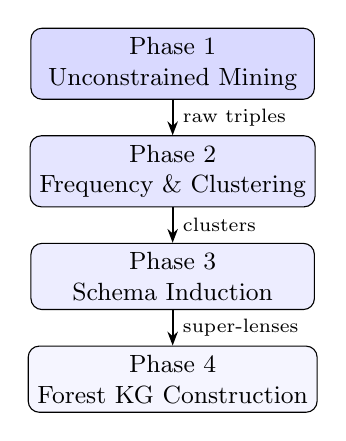
\begin{tikzpicture}[
  box/.style={draw, rounded corners=4pt, fill=gray!10,
              minimum width=3.6cm, minimum height=0.7cm,
              font=\small, align=center},
  arr/.style={-{Stealth[length=5pt]}, thick},
  node distance=0.45cm
]
\node[box, fill=blue!15] (p1) {Phase 1\\Unconstrained Mining};
\node[box, fill=blue!10, below=of p1] (p2) {Phase 2\\Frequency \& Clustering};
\node[box, fill=blue!7,  below=of p2] (p3) {Phase 3\\Schema Induction};
\node[box, fill=blue!4,  below=of p3] (p4) {Phase 4\\Forest KG Construction};
\draw[arr] (p1) -- node[right, font=\scriptsize]{raw triples} (p2);
\draw[arr] (p2) -- node[right, font=\scriptsize]{clusters} (p3);
\draw[arr] (p3) -- node[right, font=\scriptsize]{super-lenses} (p4);
\end{tikzpicture}
\caption{Four-phase data-driven schema induction pipeline.}
\label{fig:pipeline}
\end{figure}

\subsection{Phase 1: Unconstrained Triple Mining}

Each dataset entry is sent to Qwen2.5-7b running locally via Ollama —
at zero API cost.
The system prompt contains \emph{no schema}: no levels, no edge type list,
no domain taxonomy.
It instructs the model only to extract whatever entities and relationships
it naturally sees, using any descriptive language that fits:

\begin{quote}
\small\textit{``Extract every entity and relationship you see.
Use natural, descriptive labels --do not force categories.
Relation: a natural descriptive phrase. Use whatever words best describe
the connection.''}
\end{quote}

Results are streamed entry-by-entry to a JSONL file, making the run
safely resumable.
Running 2,500 entries on Apple Silicon M-series hardware takes approximately
2.5--3 hours.

\subsection{Phase 2: Frequency Analysis and Clustering}

We collect all extracted triples and count:
\begin{itemize}
\item \textbf{Entity frequency}: how often each entity label appears
  as a head or tail across all triples.
\item \textbf{Relation frequency}: how often each relation phrase appears.
\item \textbf{Pathway frequency}: how often each (head, relation, tail)
  pattern recurs --a proxy for cultural salience.
\end{itemize}

Entity and relation labels are then clustered using TF-IDF character
n-gram vectors (2--4 grams) with DBSCAN
($\varepsilon = 0.40$ for relations, $0.35$ for entities).
DBSCAN requires no pre-specified number of clusters --the data determines
how many groups emerge.
Each cluster receives a canonical label equal to its most-frequent member.

\paragraph{Level assignment.}
Rather than assigning levels by design, we derive them from frequency.
Entity clusters are sorted by total frequency; Jenks natural breaks
\cite{jenks1967datamodel} on the log-frequency distribution identify
tier boundaries automatically.
High-frequency clusters become high-abstraction (low-level) nodes;
low-frequency clusters become specific leaf nodes.
The number of levels is not fixed --the data decides.

\subsection{Phase 3: Schema Induction (Lens Discovery)}

Relation clusters are the central artifact of our method.
Each relation cluster represents a distinct \emph{type} of cultural
relationship that the data itself identified.
We call these clusters \textbf{lenses}: each lens is a perspective through
which cultural knowledge can be read.

For each lens, we collect:
\begin{itemize}
  \item All relation phrases that belong to it (the edge vocabulary);
  \item The most frequent entity pairs connected by relations in this lens;
  \item The coverage (number of triples explained by this lens).
\end{itemize}

Lenses with coverage below a threshold (default: 10 triples) are discarded
as noise.
The remaining lenses are optionally meta-clustered at a higher
$\varepsilon$ to merge near-synonym lenses before the final extraction step.

\subsection{Phase 4: Forest Knowledge Graph Construction}

Using the induced lens schema, we run a \emph{second} structured
extraction pass over the same dataset entries.
This time, the system prompt presents the data-derived lenses and asks the
model to classify each entry according to which lenses apply and extract
nodes and edges accordingly.
For each lens, we assemble a knowledge graph using the entity clusters
(with their frequency-derived levels) as nodes and the lens's relation
phrases as edge labels.

The output is a \textbf{forest of knowledge graphs} --one per lens —
stored separately in \texttt{outputs/final/graphs/lens\_\textit{N}/}.
This structure naturally encodes the multi-dimensional nature of cultural
knowledge: the same cultural practice may appear in multiple graphs
(e.g., a food prohibition appears in both the \emph{values} graph and the
\emph{avoid} graph), representing its multiple cultural meanings.

%% ============================================================
\section{Results}
\label{sec:results}

\subsection{Mining Statistics}

Table~\ref{tab:mining} summarizes Phase~1 results.

\begin{table}[h]
\centering
\small
\begin{tabular}{lr}
\toprule
\textbf{Metric} & \textbf{Value} \\
\midrule
Dataset entries processed     & 2,500 \\
Raw triples extracted         & 8,700 \\
Avg.\ triples per entry       & 3.5 \\
Unique entity labels          & 8,405 \\
Unique relation phrases       & 4,189 \\
\midrule
Entity clusters (after dedup) & 257 \\
Relation clusters             & 126 \\
Lenses (coverage $\geq$ 10)  & 74 \\
\bottomrule
\end{tabular}
\caption{Phase 1--2 mining and clustering statistics.}
\label{tab:mining}
\end{table}

\subsection{Discovered Lenses}

Table~\ref{tab:lenses} shows the 20 highest-coverage lenses.
These were not designed --they emerged entirely from frequency patterns in
the data.

\begin{table}[h]
\centering
\small
\begin{tabular}{clr}
\toprule
\textbf{Rank} & \textbf{Lens name} & \textbf{Coverage} \\
\midrule
1  & uses              & 886 \\
2  & performed during  & 573 \\
3  & values            & 276 \\
4  & includes          & 207 \\
5  & features          & 200 \\
6  & practices         & 168 \\
7  & involves          & 128 \\
8  & hosts             & 119 \\
9  & symbolizes        & 114 \\
10 & vary by           & 114 \\
11 & prefer            & 112 \\
12 & originates from   & 108 \\
13 & engage in         & 106 \\
14 & enjoy             & 97  \\
15 & prepares          & 94  \\
16 & reflects          & 76  \\
17 & characterized by  & 73  \\
18 & associated with   & 72  \\
19 & participate in    & 71  \\
20 & known for         & 64  \\
\bottomrule
\end{tabular}
\caption{Top 20 discovered lenses by triple coverage.}
\label{tab:lenses}
\end{table}

\paragraph{Unexpected lenses.}
Beyond the high-coverage lenses, several low-coverage but culturally
significant lenses emerged that no hand-crafted schema would have included:

\begin{itemize}
  \item \textbf{struggle with} (cov.\ 12): captures cultural tension,
  generational conflict, and identity negotiation --dimensions entirely
  absent from schema-first graphs.
  \item \textbf{eats together} (cov.\ 17): communal food practices as a
  distinct cultural dimension, separate from food prohibition or
  food production.
  \item \textbf{narrates} (cov.\ 10): oral tradition and storytelling as
  cultural transmission.
  \item \textbf{woven in} (cov.\ 33) and \textbf{wear} (cov.\ 37):
  material culture and textile identity as standalone dimensions.
  \item \textbf{avoid} (cov.\ 11): cultural taboo and prohibition, richer
  than the single \emph{restricts} edge type in Task~1.
\end{itemize}

\subsection{Comparison with Schema-First Baseline}

Table~\ref{tab:comparison} directly compares the two approaches.

\begin{table*}[t]
\centering
\small
\begin{tabular}{lll}
\toprule
\textbf{Property} & \textbf{Task 1 (Schema-First)} & \textbf{Task 2 (Data-Driven)} \\
\midrule
Schema source         & Hand-designed before data     & Induced from data \\
Edge type vocabulary  & 8 types (fixed)               & 74 lenses, 4,189 phrases \\
Level structure       & 5 levels (fixed)              & Frequency-derived (data decides) \\
Cross-domain edges    & Rare, incidental              & First-class (each lens crosses domains) \\
Graph structure       & 1 monolithic graph            & Forest of 67 graphs \\
Nodes / Edges (total) & 7,542 / 8,639                 & TBD (pending final run) \\
Dominant edge type    & \emph{manifests\_in} (70.3\%) & Distributed across 74 lenses \\
LLM                   & Claude Haiku (API)            & Qwen2.5-7b (local, free) \\
API cost              & $\sim$\$10                    & \$0 \\
Missing dimensions    & tension, taboo, communality   & All present \\
\bottomrule
\end{tabular}
\caption{Comparison of schema-first (Task~1) and data-driven (Task~2) approaches.}
\label{tab:comparison}
\end{table*}

\paragraph{Key finding.}
The schema-first approach produced a graph dominated by a single structural
edge (\emph{manifests\_in}, 70.3\%) because the 8 fixed types were
insufficient to capture the actual diversity of cultural relations.
The data-driven approach reveals that cultural knowledge organizes itself
along at least 74 distinct relational dimensions --a 9$\times$ richer
vocabulary --and that many of the most culturally meaningful dimensions
(tension, taboo, communal practice, oral tradition) would never have been
included in a hand-crafted schema.

%% ============================================================
\section{Discussion}
\label{sec:discussion}

\paragraph{The forest as a cultural reasoning substrate.}
Each lens graph encodes a specific perspective on cultural knowledge.
A scenario involving food can be simultaneously read through the
\emph{values} graph (what the food practice expresses), the
\emph{avoid} graph (what is prohibited), the \emph{eats together} graph
(who shares the practice), and the \emph{originates from} graph (its
historical roots).
This multi-graph structure naturally supports the parallel cultural
reasoning pathways that motivate our project: an expert model can traverse
multiple lens graphs simultaneously, producing culturally diverse responses
rather than a single dominant answer.

\paragraph{Frequency as a proxy for cultural salience.}
By using triple frequency to derive both entity levels and lens importance,
we operationalize cultural salience computationally.
A practice that appears in thousands of dataset entries across multiple
cultural groups is genuinely cross-cultural and rises to a high-abstraction
node. A practice that appears in a handful of entries from one region
becomes a leaf node specific to that community.
This frequency-derived structure is more empirically grounded than any
manually assigned taxonomy.

\paragraph{Limitations.}
The TF-IDF character n-gram clustering cannot merge semantically equivalent
but orthographically distinct relations (e.g., \emph{symbolizes} $\approx$
\emph{represents} $\approx$ \emph{depicts}).
A future improvement is to replace TF-IDF with semantic embeddings
(e.g., via a local embedding model) for the relation clustering step.
Additionally, the average of 3.5 triples per entry is below our target of
4--10, suggesting the mining prompt could be strengthened.

%% ============================================================
\section{Next Steps}
\label{sec:next}

\begin{enumerate}
  \item \textbf{Final KG construction}: Run Phase~4 on all 2,500 entries
  to produce the complete forest of 67 knowledge graphs using the
  data-derived schema.
  \item \textbf{Semantic embedding clustering}: Replace TF-IDF with
  local semantic embeddings to achieve better lens consolidation.
  \item \textbf{Philosopher validation}: Compare discovered lenses against
  philosophical and anthropological frameworks for cultural categorization
  (e.g., work on cultural ontologies from the University of Waterloo).
  \item \textbf{Cross-lens edges}: Construct edges \emph{between} lens
  graphs to capture how cultural dimensions interact (e.g., how the
  \emph{religion} lens and the \emph{food} lens are connected).
  \item \textbf{Recursive agentic framework}: Build an expert model that
  traverses the forest to generate multi-path, culturally diverse responses
  to arbitrary scenarios.
\end{enumerate}

%% ============================================================
\section{Related Work}
\label{sec:related}

\citet{tonga2026llms} extract cultural commonsense knowledge graphs from
LLM pretraining data. Their approach uses a fixed ontology; ours induces
the ontology from the data itself.
\citet{nguyen2023candle} provide the largest cultural commonsense KB;
we repurpose it as a mining corpus rather than a benchmark.
\citet{shi2024culturebank} demonstrate that behavioral norms can be
extracted from social media; we extend this to cross-dataset schema
discovery.
\citet{myung2024blend} show that LLMs fail on culturally diverse QA;
our forest structure is designed to address this failure mode by
providing multi-path cultural reasoning pathways.

%% ============================================================
\bibliography{references}

\appendix

\section{Full Lens List}
\label{app:lenses}

\begin{table}[h]
\centering
\small
\begin{tabular}{clr}
\toprule
\textbf{ID} & \textbf{Lens} & \textbf{Coverage} \\
\midrule
0  & uses              & 886 \\
1  & performed during  & 573 \\
2  & values            & 276 \\
3  & includes          & 207 \\
4  & features          & 200 \\
5  & practices         & 168 \\
6  & involves          & 128 \\
7  & hosts             & 119 \\
8  & symbolizes        & 114 \\
9  & vary by           & 114 \\
10 & prefer            & 112 \\
11 & originates from   & 108 \\
12 & engage in         & 106 \\
13 & enjoy             & 97  \\
14 & prepares          & 94  \\
15 & reflects          & 76  \\
16 & characterized by  & 73  \\
17 & associated with   & 72  \\
18 & participate in    & 71  \\
19 & known for         & 64  \\
20 & is                & 54  \\
21 & receives          & 53  \\
22 & promotes          & 48  \\
23 & part of           & 48  \\
24 & produces          & 43  \\
25 & marks             & 42  \\
26 & made from         & 42  \\
27 & encourage         & 41  \\
28 & consume           & 38  \\
29 & expressed through & 38  \\
30 & requires          & 37  \\
31 & focuses on        & 36  \\
32 & experience        & 34  \\
33 & woven in          & 33  \\
34 & depicts           & 30  \\
35 & shares            & 30  \\
36 & play with         & 30  \\
37 & represents        & 29  \\
38 & combines          & 29  \\
39 & provide           & 28  \\
40 & wear              & 25  \\
41 & prioritizes       & 25  \\
42 & follow            & 25  \\
43 & influences        & 24  \\
44 & emphasizes        & 23  \\
45 & honors            & 21  \\
46 & perceived as      & 20  \\
47 & type of           & 19  \\
48 & consists of       & 19  \\
49 & contains          & 19  \\
50 & inspired by       & 18  \\
51 & material          & 18  \\
52 & cause             & 18  \\
53 & offer             & 17  \\
54 & eats together     & 17  \\
55 & result of         & 17  \\
56 & support           & 15  \\
57 & accompanied by    & 15  \\
58 & seek              & 14  \\
59 & ensures           & 14  \\
60 & expect            & 14  \\
61 & struggle with     & 12  \\
62 & displays          & 12  \\
63 & affects           & 12  \\
64 & applied to        & 12  \\
65 & exhibits          & 11  \\
66 & avoid             & 11  \\
67 & attributed to     & 11  \\
68 & narrates          & 10  \\
69 & seen as           & 10  \\
70 & integral to       & 10  \\
71 & weaves            & 10  \\
\bottomrule
\end{tabular}
\caption{All 72 discovered lenses with triple coverage.}
\label{tab:all_lenses}
\end{table}

\end{document}
